% shell-escape
\documentclass[12pt]{article}
\usepackage[shorthands=off,czech]{babel}
\usepackage[T1]{fontenc} 
\usepackage[utf8]{inputenc}
\usepackage{minted}
\usepackage{xurl}
\usepackage{graphicx}
\usepackage[binary-units=true, output-decimal-marker={,}]{siunitx}
\usepackage{tikz}
\usepackage{placeins}
\newcommand{\twi}{I\textsuperscript{2}C}
\usetikzlibrary{chains,decorations.pathreplacing}




\title{Programování hada na mikrokontroléru K64F}
\date{}

%TODO: modifikace knihovny
%TODO: jaky uzivatel?
%TODO: bude mit pristup k tty?

\begin{document}
\sloppy
\maketitle

%\section*{Cíl dneška}
Dnešním cílem bude naprogramovat hru hada na mikrokontroléru K64F s architekturou ARM.
Na rozšířující desce je barevný LCD displej o rozměrech $320 \times 240$ pixelů a tlačítka, kterými se bude had ovládat.
Na vývojové desce je k dispozici akcelerometr, a proto budeme na závěr implementovat i jednoduché ovládání pomocí naklápění.

\begin{figure}[h]
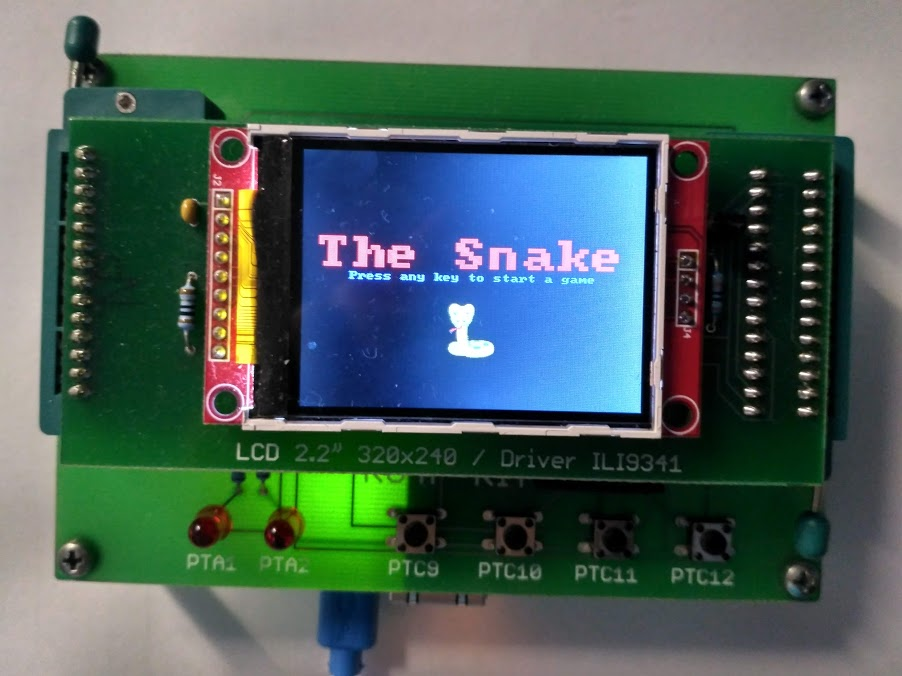
\includegraphics[width=\linewidth]{figures/snake}
\end{figure}


% Procesor má k dispozici \SI{1}{\mega \byte} pro kod programu a \SI{256}{\kilo \byte} RAM paměti.


\section{Zprovoznění vývojového prostředí}
\subsection{Stáhnutí projektu}
Na adrese \url{http://linedu.vsb.cz/~trn0038/snake/thesnake.tar.gz} je k dispozici připravený projekt s LCD knihovnou a knihovnou pro akcelerometr.
Knihovnu si stáhneme a někam rozbalíme.

Stáhnutí a rozbalení také můžeme provést i v terminálu:
\begin{minted}{shell-session}
$ wget http://linedu.vsb.cz/~trn0038/snake/thesnake.tar.gz
$ tar -xf thesnake.tar.gz
$ cd thesnake 
\end{minted}

Alternativně si můžeme stáhnout projekt z Gitu:
\begin{minted}{shell-session}
$ git clone http://linedu.vsb.cz/~trn0038/snake/thesnake.git
$ cd thesnake
\end{minted}

\subsection{Import projektu do MCUXpresso}
Hada budeme programovat v programu MCUXpresso.
Po spuštění naimportujeme rozbalený projekt.
Vybereme \texttt{File -> Import} a zvolíme \texttt{General -> Existing Projects into Workspace}.

\subsection{Nahrání kódu do mikrokontroléru a ladění}
Kod nahrajeme do mikrokontroléru pomocí modré ikonky:

\begin{center}
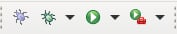
\includegraphics{figures/blue-debug.jpg}
\end{center}

Program lze efektivně ladit pomocí debuggeru nebo pomocí \mintinline{c}{printf}.
Výpisy jsou pak dostupné:
\begin{minted}{shell-session}
$ minicom -D /dev/ttyUSB0 -b 9600
\end{minted}
Program lze ukončit stisknutím \textsc{CTRL+A} následovaný klávesou \textsc{X}.

\subsection{Knihovna Mbed 2}
Knihovna Mbed 2 má k dispozici několik tříd pro snadné použití periférií.
Hlavíčkové soubory tříd jsou k dispozici v adresáři projektu \texttt{mbed/drivers} nebo online\footnote{\url{https://os.mbed.com/users/mbed_official/code/mbed/file/65be27845400/drivers/}}.
K dispozici je i dokumentace s ukázkami \url{https://os.mbed.com/handbook/Homepage}.
Detailnější informace lze nalézt v dokumentu \url{http://poli.cs.vsb.cz/edu/apps/lab/apps-labexc.pdf}.

\section{Vykreslení čtverce na LCD displeji}
LCD displej je k mikrokontroléru připojen pomocí SPI rozhrání, a posílame příkazy nebo jednotlivé pixely do paměti řadiče displeje.
Základní komunikace s displejem je naimplementovaná v knihovně \texttt{lcd\_lib.cpp}.
Dostupné funkce lze nalézt v hlavičkovém souboru \texttt{lcd\_lib.h}.

Had se bude pohybovat po políčkach o velikosti například $4\times4$ pixelů.
Proto prvním úkolem bude vytvořit funkci, která konkrétní políčko vyplní nějakou barvou.
Prototyp takové funkce by mohl být například:
\begin{minted}{c}
void fill_rect(int x, int y, uint16_t color);
\end{minted}
Vykreslení čtverce budeme provádět po pixelech pomocí funkce \mintinline{c++}{void LCD_put_pixel(int x, int y, int color)}.

Displej si ukládá barvy v 16bitovém formátu 5:6:5 (R, G, B), kde jednotlivá čísla značí kolik bitů využívá daná barva.
V tomto případě tedy červená chce 5 bitů, zelená 6 bitu a modrá 5 bitů.
Zelená má o bit navíc, poněvadž na zelenou barvu je lidské oko citlivější.
Dále si můžeme vytvořit funkci, která  pro standardní RGB formát 8:8:8 vytvoří 16bitovou hodnotu ve formátu 5:6:5 dle obrázku~\ref{fig:rgb565}.
Prototyp takové funkce může být následující:
\begin{minted}{c}
uint16_t to_color(uint8_t r, uint8_t g, uint8_t b);
\end{minted}

\begin{figure}[ht]
	\centering
    \begin{tikzpicture}[
node distance=0pt,
 start chain = A going right,
    X/.style = {rectangle, draw,% styles of nodes in string (chain)
                minimum width=2ex, minimum height=3ex,
                outer sep=0pt, on chain},
    B/.style = {decorate,
                decoration={brace, amplitude=5pt,
                pre=moveto,pre length=1pt,post=moveto,post length=1pt,
                raise=1mm,
                            #1}, % for mirroring of brace, if necessary
                thick},
    B/.default=mirror, % by default braces are mirrored
                    ]
\foreach \i in {1,1,1,1,1} \node[X, fill=red] {\i};
\foreach \i in {0,0,0,0,0,0} \node[X, fill=green] {\i};
\foreach \i in {1,1,1,1,1} \node[X, fill=blue] {\i};
    \end{tikzpicture}
	\caption{Barevný format 5:6:5}
  \label{fig:rgb565}
\end{figure}

Nejprve je potřeba jednotlivým složkám změnit rozsah bitů.
Pro červenou barvu změníme rozsah z $0 - 255 (2^8-1)$ na $0 - 31 (2^{5}-1)$.

Poté se mohou vložit na konkrétní pozici v 16bit čísle pomocí bitového posunu a logického operátoru OR (v C se zapisuje \texttt{|}).

Operátor bitového posunu doleva (\mintinline{c++}{a << b}) posune bity čísla \texttt{a} o \texttt{b} pozic v binárním zápise doleva.
Například posunutí čísla $5$ o dvě místa může vypadat následovně:
\begin{minted}{c}
uint8_t num = 5;                 // bin:   101
uint8_t num_shifted = num << 2;  // bin: 10100
\end{minted}


\section{Posun hada}
Pro souřadnici $x$, $y$ je vhodné si udělat vlastní datový typ:
\begin{minted}{c}
typedef struct {int x, y; } Vector2;
\end{minted}

Had se posunuje tak, že ocas se posune na článek před ocasem, článek před ocasem se posune na třetí článek od konce atd.
Hlava se pak posune na nové a prázné políčko.
Protože jsou všechny články hada stejné, tak nemusíme nic přesouvat, ale stačí zrušit akuální ocas a přidat novou hlavu o poličko dopředu v aktuálním směru.
Tato struktura připomíná frontu, ale my si jej naimplementujeme pomocí pole.
Pro zjednodušení využijeme \mintinline{c++}{std::vector}, do kterého budeme ukládat souřadnice datového typu \mintinline{c++}{Vector2}.

Had se bude v každé iteraci hry posunovat v jeho aktuálním směru.
Takže k aktuální pozici hlavy přičteme směr a přidáme na konec vektoru s hadem.
Tuto hlavu také musíme vykreslit pomocí funkce \mintinline{c++}{fill_rect}.
Následně se musí ocas odstranit z vektoru hada a na displej vykreslit černou barvu.

Na konci iterace je vhodné dat nějakou pauzu.
V této fázi by se měl had sám posouvat v jednom směru.
Při dosaženi okraje se had může objevit na protější straně.

\section{Ovládání hada tlačítky}
Hada budeme ovládat pomocí čtyř tlačítek.
Stav tlačítka zjistíme přečtením hodnoty na pinu.
Schéma zapojení můžeme vidět na obrázku~\ref{fig:button}.
V normálním stavu je tlačítko rozpojeno a tak na pinu vidíme logickou jedničku.
Pokud se tlačitko sepne, tak na pinu uvidíme logickou nulu.

\begin{figure}[ht]
\centering
  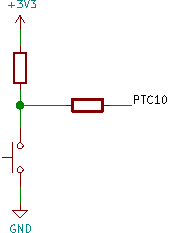
\includegraphics[width=4cm]{figures/button}
\caption{Schéma zapojení tlačítka}
 \label{fig:button}
\end{figure}
\FloatBarrier

Pro přečtení hodnoty na pinu můžeme využít třídu \mintinline{c++}{DigitalIn}, jejiž argumentem je název pinu, který je vytištěn hned pod tlačítkem.
Aktuální hodnotu pinu v daném okamžiku si můžeme vytisknout pomocí:
\begin{minted}{c}
DigitalIn left(PTC9);
printf("%d\r\n", left)
\end{minted}

Pokud bychom četli stavy všech tlačítek v jednom okamžiku v každém cyklu hry, tak bychom nějaké stisky nebyli schopni vůbec zaznamenat. 

Abychom nemuseli aktivně kontrolovat, zda došlo ke stisku tlačítka, tak můžeme nastavit, aby nás mikrokontrolér sám informoval o tom, že proběhla změna na pinu.
Změna může být například náběžná hrana, kdy se stav logické hodnoty změní z nuly na jedničku.
Podobně je to pro sestupnou hranu.
K pinům můžeme přiřadit funkci, která se zavolá při dané události.
V této funkci můžeme například přečíst hodnotu na pinu jako jsme to dělali doposud.
Místo třídy \mintinline{c++}{DigitalIn} musíme využít \mintinline{c++}{InterruptIn} a zaregistrovat funkci pomocí \mintinline{c++}{fall} či \mintinline{c++}{rise}.
Funkce nesmí mít žádný parametr a také nic vracet.
Ve funkci můžeme přečíst stavy všech tlačítek, jako jsme to dělali doposud - akorát s tím rozdílem, že budeme kontrolovat stav hned při změně.

V hlavní smyčce programu můžeme z uložené klávesy změnit směr hada a třeba přidat podmínky, aby se nemohl otočit čelem vzad.

\section{Generování jablek a růst hada}
Náhodně vygenerujem souřadnice jablka, uložíme do globalní proměnné a vykreslíme.
Pokud se hlava hada dostane na souřadnici jablka tak, nebudeme odstraňovat ocas hada.
Tím se had prodlouží o jeden článek.
Po sežrání se může zvýšit čítač skóre.

Platnost jablka můžeme časově omezit čítačem, který se inkrementuje v každé iteraci hry.
Po dosažení určité hodnoty vygenerujeme jablko na nové pozici.

Bylo by také vhodné ošetřit, aby se jablko nevygenerovalo na hadovi.

\section{Ovládání hada pomocí akcelerometru}
Hada můžeme alternativně ovládat pomocí náklápění.
Vývojová deska obsahuje senzor s akcelerometrem, který vrací zrychlení ve všech třech osách.
Senzor je připojen k mikrokontroléru pomocí sběrnice \twi{} a využívá adresu \texttt{FXOS8700CQ\_SLAVE\_ADDR1}.
Sensor je při resetu vypnutý, aby šetřil energii.
Inicializace akcelerometru může vypadat následovně:
\begin{minted}{c}
I2C i2c(PTE25, PTE24);
FXOS8700QAccelerometer acc(i2c, FXOS8700CQ_SLAVE_ADDR1);
acc.enable();
\end{minted}

Zrychlení můžeme ze senzoru přečíst následovně:
\begin{minted}{c++}
motion_data_units_t acc_data;
acc.getAxis(acc_data);
printf("%f %f %f\r\n", acc_data.x, acc_data.y, acc_data.z);
\end{minted}
Ve vodorovné poloze získáme hodnoty přibližně $ x = 0$, $y = 0$ a $z = 9,81 $.
Orientaci os lze vidět na obrázku~\ref{fig:axes}.

\begin{figure}[ht]
  \centering
  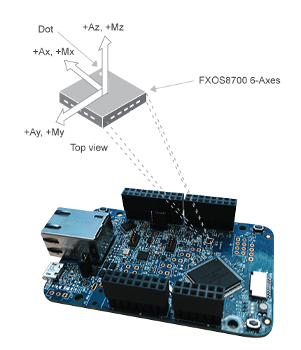
\includegraphics[width=7cm]{figures/axis}
  \caption[]{Orientace os akcelerometru na vývojové desce\footnotemark}
  \label{fig:axes}
\end{figure}
\footnotetext{\url{https://www.mathworks.com/help/supportpkg/freescalefrdmk64fboard/ref/fxos87006axessensor.html}}

Směr hada můžeme jednoduše změnit pokud se hodnota v ose dostane přes nějaký práh.

\section{Kousnutí hada}
Hra končí pokud se had kousne do jednoho článku.
Tuto skutečnost můžeme ověřit tak, že nová hlava se nevyskytuje ve vektoru hada.
Pokud hra skončí, tak můžeme počkat na stisk tlačítka a následně resetovat stav celé hry a začít znovu.

\section{Překážky}
Lze implementovat podobně jako v předchozím bodě.

\section{Hlavní menu a konec hry}
Pro vypisování textu na displej jsou připravené tři funkce.
Souřadnice \texttt{x}, \texttt{y} udává konkrétní pixel displeje a nijak nesouvisi s políčky hada.
Písmo textu je proporcionální, což znamená, že každé písmeno zabírá stejnou šířku a zjednodušují se nám výpočty, např. při centrování textu na střed displeje.
Parametr \texttt{scale} udává kolik pixelů na šířku/výšku zabere jeden bod písma.
Rozumné hodnoty jsou od 1 do 3.


\begin{minted}{c}
// print single char
void LCD_print_char(int x, int y, int scale, uint16_t color, char c);

// print string
void LCD_print(int x, int y, int scale, uint16_t color, const char *msg, ...);

// print centered string
void LCD_print_centered(int y, int scale, uint16_t color, const char *msg, ...);
\end{minted}

Funkce \texttt{LCD\_print} vytiskne na daný pixel řetězec, který je možné i naformátovat jako u funkce \texttt{printf}.

Na konci hry se může například vykreslit \textit{Game over} a skóre s počtem sežraných jablek.

\section{Vykreslení obrázku}
Formáty jako PNG či JPEG ukládaji obrázek v komprimované podobě a bylo by potřeba další knihovny.
Proto může být vhodné připravit obrázek v 16bit formátu 5:6:5.
K mikrokontroléru nemáme připojenou žádnou pamětovou kartu a proto musíme obrázek umístit přímo do programu.
Následujícimi příkazy můžeme z obrázku \texttt{input.jpg} vygenerovat hlavíčkový soubor \texttt{logo.h}:
\begin{minted}{shell-session}
# změna velikosti obrázku na 64x64
$ convert input.jpg -resize 64x64 resized.bmp

# získaní skutečných rozměrů
$ width=$(identify -format %w "resized.bmp")
$ height=$(identify -format %h "resized.bmp")

# převod na formát BMP RGB565 a extrakce pixelů
$ convert resized.png +flip -define bmp:subtype=RGB565 bmp2:- | \
  tail -c $((width*height*2)) > raw_rgb565

# vygenerování hlavičkového souboru
$ xxd -i raw_rgb565 > logo.h 
$ echo "const int raw_rgb565_width = $width;" >> logo.h
$ echo "const int raw_rgb565_height = $height;" >> logo.h
\end{minted}

Ve vygenerovaném souboru je proměnná \texttt{raw\_rgb565}.
Pro vykreslení stačí pole projít po 16 bitech (přetypujem na \mintinline{c++}{uint16_t}) a postupně vykreslit po řádcích.

\section{Ovládání hada z počítače}
Hada můžeme ovládat z počítače pomocí klávesnice.
Nejjednodušeji toho můžeme docílit ve skriptovacím jazyce Python.
Po stisku klávesy se pošle přes sériovou linku znak, který na straně procesu přečteme a změníme směr hada.

\noindent
\begin{minipage}{\linewidth}
Kód na straně počítače může vypadat následovně:
\inputminted{python}{control.py}
  \vspace{0.3cm}
\end{minipage}
Skript uložíme do nějakého souboru a můžeme spustit pomocí:
\begin{minted}{shell-session}
$ python control.py
\end{minted}
Program můžeme ukončit zkratkou \textsc{CTRL+C}.

Na straně K64 můžeme přečíst znak následovně:
\begin{minted}{c++}
if(pc.readable()) {
  if(pc.getc() == 'l') {
    // jdi doleva
  }
}
\end{minted}

\section{Vlastní implementace struktury hada}
Použití \texttt{std::vector} nemusí být vhodné, protože provádí dynamickou alokaci a samotná implementace také zvětšuje velikost kódu.
Nemusí ani pomoct kompilace se zapnutou optimalizací velikosti programu.
Například při použití \texttt{std::vector} došlo ke zvětšení kódu z \SI{1.4}{\kilo\byte} na \SI{83.9}{\kilo \byte}:
\begin{verbatim}
   text    data     bss     dec     hex filename
   1472    1084      28    2584     a18 nostl
  83945    2500     128   86573   1522d vector
\end{verbatim}
Toto však může být problém, protože mikrokontrolér má k dispozici pouze \SI{1024}{\kilo\byte} pro program.

Strukturu hada můžeme naimplementovat jako kruhové statické pole se dvěma indexy.
První index určuje pozici hlavy a druhý index pozici ocasu.

\end{document}
